\chapter{Introduction to Computational Science}

\section{Learning Objectives}

Upon completion of this chapter, students should be able to:

\begin{enumerate}
  \item Define computational science and explain its interdisciplinary nature
  \item Identify the three pillars of computational science and understand their interconnected relationship
  \item Understand the role of computational thinking in problem-solving across various domains
  \item Recognize applications of computational science across diverse fields including physics, biology, economics, and engineering
  \item Distinguish between different types of computational models and their appropriate applications
  \item Explain the computational science workflow and methodology for systematic problem-solving
  \item Appreciate the tripartite approach that distinguishes computational science from traditional scientific methods
  \item Understand how computational science bridges theoretical and experimental approaches to scientific inquiry
\end{enumerate}

\begin{figure}[ht]
  \centering
  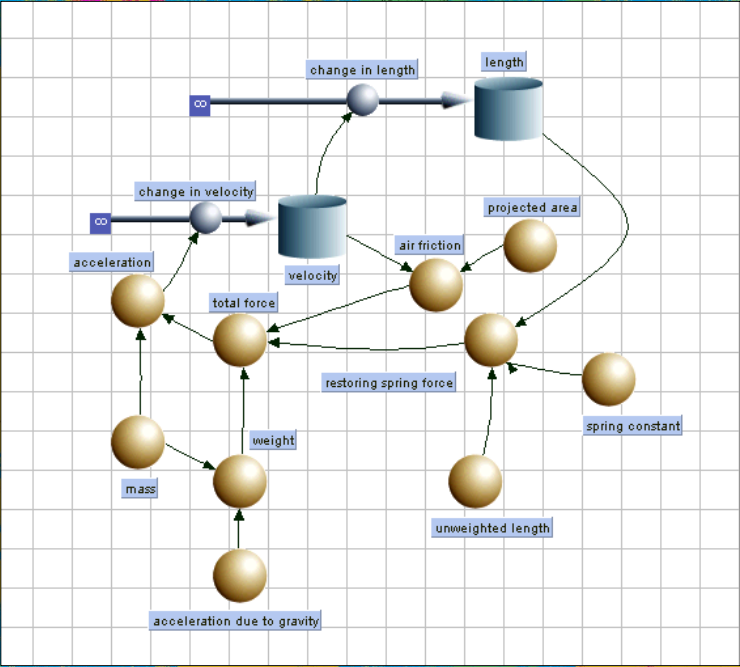
\includegraphics[width=0.8\textwidth]{images/chapter1_title_simulation.png}
  \caption{Mass-Spring Dynamics Simulation}
  \label{fig:chapter1_title}
\end{figure}

Figure~\ref{fig:chapter1_title} shows the computational modeling of a physical system with interconnected masses, springs, and forces including gravity, air friction, and restoring forces.

\section{Mass-Spring Dynamics Simulation}

\subsection{What is Mass-Spring Dynamics?}

\begin{conceptcard}{Mass-Spring Dynamics Definition}
\textbf{Mass-Spring Dynamics} is a fundamental physical and computational model that describes the behavior of systems consisting of point masses connected by elastic springs. This model serves as a cornerstone in physics, engineering, and computational science for understanding oscillatory motion, mechanical vibrations, and complex multi-body systems.
\end{conceptcard}

Mass-Spring Dynamics represents one of the most important and widely applicable models in computational physics. At its core, it describes how objects with mass respond to forces, particularly the restoring forces exerted by springs and the influence of external forces such as gravity and friction.

\subsubsection{Fundamental Components of Mass-Spring Systems}

A mass-spring system consists of several key elements that work together to create complex dynamic behaviors:

\begin{enumerate}
    \item \textbf{Point Masses}: These represent objects with mass but negligible size, characterized by:
    \begin{itemize}
        \item Mass value (m) that determines inertial properties
        \item Position coordinates (x, y, z) in space
        \item Velocity components that describe motion
        \item Acceleration determined by applied forces
    \end{itemize}
    
    \item \textbf{Springs}: Elastic connectors that exert forces proportional to displacement:
    \begin{itemize}
        \item Spring constant (k) indicating stiffness
        \item Natural (rest) length when no force is applied
        \item Current length based on connected mass positions
        \item Restoring force that opposes deformation
    \end{itemize}
    
    \item \textbf{External Forces}: Environmental influences affecting the system:
    \begin{itemize}
        \item Gravitational acceleration pulling masses downward
        \item Air resistance opposing motion
        \item Applied forces from user interaction or external sources
        \item Constraint forces maintaining system integrity
    \end{itemize}
    
    \item \textbf{Damping Elements}: Energy dissipation mechanisms:
    \begin{itemize}
        \item Viscous damping proportional to velocity
        \item Friction forces opposing motion
        \item Energy loss that causes oscillations to decay over time
    \end{itemize}
\end{enumerate}

\subsubsection{Physical Principles Governing Mass-Spring Dynamics}

The behavior of mass-spring systems is governed by fundamental laws of physics that can be expressed mathematically:

\begin{enumerate}
    \item \textbf{Newton's Second Law of Motion}:
    \begin{equation}
        \vec{F}_{net} = m\vec{a}
    \end{equation}
    where the net force on a mass determines its acceleration.
    
    \item \textbf{Hooke's Law for Elastic Springs}:
    \begin{equation}
        \vec{F}_{spring} = -k(\vec{L} - \vec{L_0})
    \end{equation}
    where:
    \begin{itemize}
        \item k is the spring constant (stiffness)
        \item $\vec{L}$ is the current spring vector
        \item $\vec{L_0}$ is the natural length vector
        \item The negative sign indicates the force opposes displacement
    \end{itemize}
    
    \item \textbf{Damping Forces}:
    \begin{equation}
        \vec{F}_{damping} = -c\vec{v}
    \end{equation}
    where c is the damping coefficient and $\vec{v}$ is the velocity vector.
    
    \item \textbf{Energy Conservation Principles}:
    \begin{itemize}
        \item Kinetic energy: $KE = \frac{1}{2}mv^2$
        \item Potential energy: $PE = \frac{1}{2}kx^2$ (for springs)
        \item Total mechanical energy in ideal systems without damping
    \end{itemize}
\end{enumerate}

\subsubsection{Applications of Mass-Spring Dynamics}

Mass-spring dynamics finds applications across numerous fields, making it a versatile and important computational model:

\begin{itemize}
    \item \textbf{Mechanical Engineering}:
    \begin{itemize}
        \item Vehicle suspension system design and analysis
        \item Vibration isolation in machinery and equipment
        \item Structural dynamics of buildings and bridges
        \item Shock absorber optimization
    \end{itemize}
    
    \item \textbf{Computer Graphics and Animation}:
    \begin{itemize}
        \item Realistic cloth and fabric simulation
        \item Hair and fur dynamics in character animation
        \item Soft body deformation in games and movies
        \item Particle system effects and simulations
    \end{itemize}
    
    \item \textbf{Robotics and Control Systems}:
    \begin{itemize}
        \item Robot arm dynamics and control
        \item Walking and running gait analysis
        \item Flexible manipulator modeling
        \item Bio-inspired locomotion systems
    \end{itemize}
    
    \item \textbf{Physics Education and Research}:
    \begin{itemize}
        \item Demonstrating oscillatory motion principles
        \item Understanding resonance and frequency response
        \item Exploring chaos and nonlinear dynamics
        \item Modeling molecular and atomic interactions
    \end{itemize}
    
    \item \textbf{Biomechanics and Medical Applications}:
    \begin{itemize}
        \item Modeling human joint and muscle dynamics
        \item Prosthetic device design and optimization
        \item Heart valve mechanics simulation
        \item Tissue elasticity and deformation studies
    \end{itemize}
\end{itemize}

\subsubsection{Computational Challenges in Mass-Spring Dynamics}

Simulating mass-spring systems computationally presents several important challenges that illustrate key concepts in computational science:

\begin{enumerate}
    \item \textbf{Numerical Integration}:
    \begin{itemize}
        \item Converting continuous differential equations to discrete time steps
        \item Choosing appropriate integration methods (Euler, Runge-Kutta, Verlet)
        \item Balancing accuracy with computational efficiency
        \item Maintaining stability over long simulation periods
    \end{itemize}
    
    \item \textbf{Time Step Selection}:
    \begin{itemize}
        \item Ensuring numerical stability with appropriate step sizes
        \item Handling stiff systems with very different time scales
        \item Adaptive time stepping for optimal performance
        \item Trade-offs between accuracy and real-time performance
    \end{itemize}
    
    \item \textbf{Force Calculation Optimization}:
    \begin{itemize}
        \item Efficient algorithms for computing spring forces
        \item Spatial data structures for neighbor finding
        \item Parallel processing for large-scale systems
        \item Memory management for complex connectivity patterns
    \end{itemize}
    
    \item \textbf{Energy Conservation and Stability}:
    \begin{itemize}
        \item Monitoring total system energy over time
        \item Preventing numerical energy gain or loss
        \item Implementing energy-conserving integration schemes
        \item Handling energy dissipation through damping
    \end{itemize}
\end{enumerate}

\subsubsection{Why Mass-Spring Dynamics is Important for Computational Science}

Mass-spring dynamics serves as an excellent introduction to computational science for several reasons:

\begin{highlightbox}{Educational Value of Mass-Spring Systems}
\begin{itemize}
    \item \textbf{Intuitive Physics}: Everyone can understand springs and masses from everyday experience
    \item \textbf{Mathematical Tractability}: Simple enough to analyze mathematically but complex enough to be interesting
    \item \textbf{Visual Appeal}: Results can be easily visualized and animated
    \item \textbf{Scalable Complexity}: Can start simple and add complexity incrementally
    \item \textbf{Interdisciplinary Connections}: Links physics, mathematics, and computer science naturally
    \item \textbf{Practical Relevance}: Has real-world applications students can relate to
\end{itemize}
\end{highlightbox}

The mass-spring model exemplifies how computational science transforms abstract mathematical concepts into concrete, observable simulations that enhance understanding and enable prediction of complex behaviors that would be difficult to analyze purely theoretically or experimentally.

\subsection{Understanding Mass-Spring Dynamics: A Computational Science Example}

Figure \ref{fig:chapter1_title} provides an excellent illustration of how computational science transforms real-world physical phenomena into mathematical models that can be simulated and analyzed computationally. This mass-spring dynamics simulation demonstrates the core principles of computational science through a tangible, observable system.

\subsubsection{The Physical System}

The mass-spring system represents one of the fundamental models in physics and engineering, consisting of:

\begin{itemize}
  \item \textbf{Point Masses}: Represented by the spherical objects in the simulation, each having specific mass properties that determine their inertial response to applied forces
  \item \textbf{Springs}: Connecting elements that exert restoring forces proportional to their displacement from equilibrium, following Hooke's Law ($F = -kx$)
  \item \textbf{Damping Elements}: Air friction and other dissipative forces that remove energy from the system over time
  \item \textbf{External Forces}: Gravitational acceleration and other environmental influences acting on the masses
\end{itemize}

\subsubsection{Mathematical Modeling Components}

The simulation incorporates several key physical principles translated into mathematical form:

\begin{enumerate}
  \item \textbf{Newton's Second Law}: $F = ma$ governs the motion of each mass, where the net force determines acceleration
      
  \item \textbf{Hooke's Law for Springs}: $F_{spring} = -k(L - L_0)$ where:
  \begin{itemize}
    \item $k$ is the spring constant (stiffness)
    \item $L$ is the current length
    \item $L_0$ is the natural (rest) length
  \end{itemize}
      
  \item \textbf{Damping Forces}: $F_{damping} = -c \cdot v$ where $c$ is the damping coefficient and $v$ is velocity
      
  \item \textbf{Gravitational Force}: $F_{gravity} = mg$ acting downward on each mass
\end{enumerate}

\subsubsection{Computational Implementation}

The simulation demonstrates how mathematical models are transformed into computational algorithms:

\begin{itemize}
  \item \textbf{Numerical Integration}: Converting continuous differential equations into discrete time steps using methods like Euler's method or Runge-Kutta algorithms
  \item \textbf{Force Calculation}: Computing the net force on each mass by summing contributions from all springs, damping, and external forces
  \item \textbf{Position Updates}: Using numerical integration to update positions and velocities at each time step
  \item \textbf{Constraint Handling}: Managing boundary conditions and connection constraints between masses
  \item \textbf{Real-time Visualization}: Rendering the dynamic system state for observation and analysis
\end{itemize}

\subsubsection{Interdisciplinary Nature Demonstrated}

This example perfectly illustrates the tripartite nature of computational science:

\begin{itemize}
  \item \textbf{Domain Science (Physics)}: Understanding of mechanics, forces, energy conservation, and material properties
  \item \textbf{Mathematical Modeling}: Translation of physical laws into differential equations and mathematical relationships
  \item \textbf{Computer Science}: Algorithm design, numerical methods, data structures for efficient computation, and visualization techniques
\end{itemize}

\subsubsection{Educational and Research Applications}

Mass-spring simulations serve multiple purposes in computational science education and research:

\begin{itemize}
  \item \textbf{Concept Demonstration}: Visualizing abstract physical principles like oscillation, resonance, and energy transfer
  \item \textbf{Parameter Studies}: Exploring how changes in mass, spring constants, or damping affect system behavior
  \item \textbf{Validation Studies}: Comparing computational results with analytical solutions for simple cases
  \item \textbf{Method Development}: Testing new numerical integration schemes and computational algorithms
  \item \textbf{Engineering Applications}: Modeling vibrations in structures, vehicle suspension systems, and mechanical assemblies
\end{itemize}

\subsubsection{Computational Challenges and Considerations}

The simulation also highlights important computational science considerations:

\begin{itemize}
  \item \textbf{Numerical Stability}: Ensuring the simulation remains stable over long time periods
  \item \textbf{Time Step Selection}: Balancing computational efficiency with accuracy
  \item \textbf{Energy Conservation}: Monitoring whether the numerical scheme preserves physical conservation laws
  \item \textbf{Performance Optimization}: Efficient algorithms for force calculations and collision detection
  \item \textbf{Scalability}: Handling systems with large numbers of interconnected masses and springs
\end{itemize}

This mass-spring dynamics example thus serves as a microcosm of computational science, demonstrating how real-world phenomena are systematically transformed into computational models that provide insights, predictions, and understanding that would be difficult or impossible to achieve through purely theoretical or experimental approaches alone.

\section{What is Computational Science?}

\begin{conceptcard}{Definition of Computational Science}
\textbf{Computational Science} is an interdisciplinary field that uses mathematical models, quantitative analysis techniques, and computer simulations to solve complex problems in science, engineering, business, and other domains. It combines the power of computing with mathematical modeling and scientific theory to understand and predict real-world phenomena through the creation and analysis of computational models.
\end{conceptcard}

Computational science represents a paradigm shift in how we approach scientific inquiry and problem-solving. Unlike traditional experimental and theoretical approaches, computational science offers a ``third pillar'' of scientific discovery that complements laboratory experiments and mathematical theory. This field has emerged as a critical component of modern research due to the increasing complexity of problems that cannot be adequately addressed through experimentation or theory alone.

The essence of computational science lies in its ability to create virtual laboratories where researchers can conduct experiments that would be impossible, too dangerous, too expensive, or too time-consuming to perform in reality. For instance, we can simulate the formation of galaxies over billions of years, model the spread of infectious diseases across populations, or test the structural integrity of buildings under various earthquake conditions.

\subsection{The Evolution of Scientific Methodology}

Historically, science has progressed through two primary approaches:

\begin{enumerate}
  \item \textbf{Empirical/Experimental Science}: Direct observation and experimentation to understand natural phenomena
  \item \textbf{Theoretical Science}: Mathematical formulation of natural laws and principles
\end{enumerate}

The 20th and 21st centuries have witnessed the emergence of a third approach—computational science—which bridges the gap between theory and experiment by enabling the exploration of complex systems through simulation and modeling.

\begin{figure}[h]
 \centering
 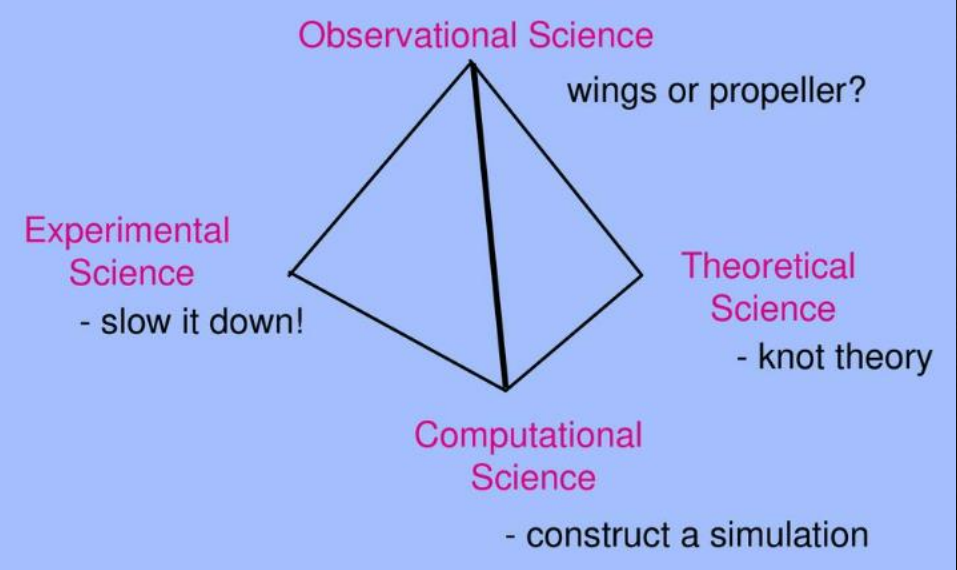
\includegraphics[width=0.8\textwidth]{images/science_four_pillars.png}
 \caption{Four Pillars of Computational Science}
 \label{fig:science_pillars}
\end{figure}

Figure~\ref{fig:science_pillars} illustrates the four complementary approaches to scientific discovery: Observational Science (observing natural phenomena), Experimental Science (controlled experiments), Theoretical Science (mathematical formulation), and Computational Science (simulation and modeling).

\subsection{The Four Pillars of Scientific Discovery}

The pyramid-shaped diagram in Figure~\ref{fig:science_pillars} represents the evolution of scientific methodology from its traditional foundations to the modern interdisciplinary approach that includes computational science. Each vertex of this pyramid represents a distinct but interconnected approach to understanding how nature behaves.

\subsubsection{Observational Science: "Wings or Propeller?"}

\begin{conceptcard}{Observational Science}
\textbf{Observational Science} involves the systematic observation and recording of natural phenomena without direct manipulation or intervention. It focuses on describing what happens in nature through careful observation and pattern recognition.
\end{conceptcard}

Observational science represents the most fundamental approach to scientific inquiry, dating back to ancient civilizations. The phrase "wings or propeller?" in the diagram captures the essence of observational science—asking questions about what we see and trying to understand the mechanisms behind observable phenomena.

\textbf{Characteristics of Observational Science:}
\begin{itemize}
    \item \textbf{Passive Data Collection}: Scientists observe and record phenomena as they naturally occur
    \item \textbf{Pattern Recognition}: Identifying trends, cycles, and relationships in observed data
    \item \textbf{Descriptive Analysis}: Cataloging and classifying natural phenomena
    \item \textbf{Hypothesis Generation}: Developing initial theories based on observations
    \item \textbf{Long-term Studies}: Monitoring changes over extended periods
\end{itemize}

\textbf{Examples of Observational Science:}
\begin{itemize}
    \item Astronomy: Observing celestial objects and cosmic phenomena
    \item Ecology: Studying animal behavior and ecosystem dynamics
    \item Meteorology: Weather pattern observation and climate monitoring
    \item Epidemiology: Disease outbreak tracking and health pattern analysis
    \item Geology: Rock formation studies and geological process observation
\end{itemize}

\subsubsection{Experimental Science: "Slow it Down!"}

\begin{conceptcard}{Experimental Science}
\textbf{Experimental Science} involves controlled manipulation of variables to test hypotheses and establish cause-and-effect relationships. The motto "slow it down!" reflects the methodical, controlled approach of experimental investigation.
\end{conceptcard}

Experimental science revolutionized our understanding of the natural world by introducing controlled conditions and systematic variable manipulation. This approach allows scientists to isolate specific factors and determine their individual effects on observed phenomena.

\textbf{Key Principles of Experimental Science:}
\begin{itemize}
    \item \textbf{Controlled Variables}: Maintaining constant conditions except for the factor being tested
    \item \textbf{Reproducibility}: Ensuring experiments can be repeated with consistent results
    \item \textbf{Isolation of Effects}: Studying one variable at a time to understand its specific impact
    \item \textbf{Statistical Analysis}: Using quantitative methods to validate results
    \item \textbf{Peer Review}: Subjecting findings to scrutiny by the scientific community
\end{itemize}

\textbf{Experimental Method Components:}
\begin{enumerate}
    \item \textbf{Hypothesis Formation}: Developing testable predictions based on observations
    \item \textbf{Experimental Design}: Planning controlled procedures to test hypotheses
    \item \textbf{Data Collection}: Gathering quantitative and qualitative measurements
    \item \textbf{Analysis and Interpretation}: Drawing conclusions from experimental results
    \item \textbf{Validation and Replication}: Confirming findings through repeated experiments
\end{enumerate}

\subsubsection{Theoretical Science: "Knot Theory"}

\begin{conceptcard}{Theoretical Science}
\textbf{Theoretical Science} involves developing mathematical models, frameworks, and abstract theories to explain natural phenomena. The reference to "knot theory" exemplifies how complex mathematical concepts can describe and predict natural behaviors.
\end{conceptcard}

Theoretical science provides the mathematical foundation for understanding natural laws and principles. It transforms observations and experimental findings into elegant mathematical formulations that can predict behavior and reveal underlying patterns.

\textbf{Components of Theoretical Science:}
\begin{itemize}
    \item \textbf{Mathematical Modeling}: Creating mathematical representations of physical phenomena
    \item \textbf{Abstract Reasoning}: Developing conceptual frameworks beyond direct observation
    \item \textbf{Predictive Capability}: Using theories to forecast future states or behaviors
    \item \textbf{Unification}: Connecting seemingly disparate phenomena under common principles
    \item \textbf{Elegance and Simplicity}: Seeking the most fundamental explanations
\end{itemize}

\textbf{Examples of Theoretical Contributions:}
\begin{itemize}
    \item Einstein's Theory of Relativity: Unified space, time, and gravity
    \item Quantum Mechanics: Mathematical description of subatomic behavior
    \item Thermodynamics: Statistical mechanics of energy and entropy
    \item Information Theory: Mathematical foundation of communication and computation
    \item Knot Theory: Mathematical study of knots with applications in DNA structure and physics
\end{itemize}

\subsubsection{Computational Science: "Construct a Simulation"}

\begin{conceptcard}{Computational Science}
\textbf{Computational Science} represents the newest pillar of scientific discovery, using computer simulations and numerical analysis to explore complex systems that are difficult to study through observation, experimentation, or pure theory alone.
\end{conceptcard}

The directive to "construct a simulation" captures the essence of computational science—creating virtual representations of real-world phenomena that can be manipulated, tested, and analyzed in ways that would be impossible with traditional approaches.

\textbf{Unique Capabilities of Computational Science:}
\begin{itemize}
    \item \textbf{Virtual Experimentation}: Conducting experiments that are impossible in reality
    \item \textbf{Scale Bridging}: Connecting phenomena across vastly different spatial and temporal scales
    \item \textbf{Parameter Exploration}: Testing thousands of scenarios rapidly and systematically
    \item \textbf{Visualization}: Making invisible phenomena visible and understandable
    \item \textbf{Prediction}: Forecasting future states based on current conditions and known laws
\end{itemize}

\textbf{Computational Approaches:}
\begin{enumerate}
    \item \textbf{Numerical Simulation}: Solving mathematical models computationally
    \item \textbf{Data Analysis}: Processing large datasets to extract patterns and insights
    \item \textbf{Machine Learning}: Using algorithms to identify patterns and make predictions
    \item \textbf{Visualization}: Creating graphical representations of complex data and phenomena
    \item \textbf{Optimization}: Finding optimal solutions to complex problems
\end{enumerate}

\subsection{The Synergistic Diamond: Integrating Four Approaches}

The diamond configuration in Figure~\ref{fig:science_pillars} is not merely a geometric arrangement—it represents the interconnected and complementary nature of these four scientific approaches. Each pillar contributes unique strengths while addressing the limitations of the others:

\begin{itemize}
    \item \textbf{Observational-Experimental Synergy}: Observations guide experimental design, while experiments validate or refute observational hypotheses
    \item \textbf{Theoretical-Computational Integration}: Theories provide the mathematical foundation for simulations, while computational results test theoretical predictions
    \item \textbf{Cross-Pillar Validation}: Findings from one approach can be validated through methods from other pillars
    \item \textbf{Complementary Perspectives}: Each approach reveals different aspects of the same natural phenomena
\end{itemize}

\begin{highlightbox}{The Power of Integration}
Modern scientific breakthroughs increasingly emerge from the integration of all four approaches:
\begin{itemize}
    \item \textbf{Climate Science}: Combines observational data, laboratory experiments, theoretical models, and computational simulations
    \item \textbf{Drug Discovery}: Integrates biological observations, controlled experiments, theoretical chemistry, and computational molecular modeling
    \item \textbf{Astrophysics}: Merges telescopic observations, laboratory plasma experiments, theoretical physics, and numerical cosmological simulations
    \item \textbf{Materials Science}: Unifies structural observations, experimental testing, theoretical solid-state physics, and computational materials design
\end{itemize}
\end{highlightbox}

\subsection{The Tripartite Nature of Computational Science}

One of the most significant aspects of computational science is its tripartite structure, which integrates three essential components into a cohesive methodology. This approach distinguishes computational science from other computational fields and establishes it as a unique scientific discipline.

\begin{conceptcard}{The Tripartite Foundation}
The \textbf{Tripartite Approach} to computational science recognizes that effective computational research requires the seamless integration of three fundamental pillars: \textbf{Architecture} (Computing Environment), \textbf{Algorithm} (Mathematical Model), and \textbf{Application} (Science). These three components work synergistically to create computational models that bridge theory and practice.
\end{conceptcard}

\subsection{Understanding the Tripartite Triangle}

\begin{figure}[h]
 \centering
 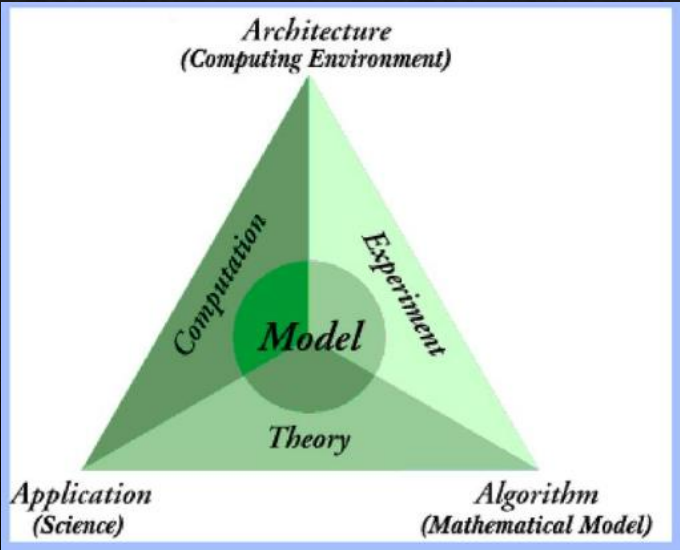
\includegraphics[width=0.7\textwidth]{images/tripartite_triangle.png}
 \caption{Tripartite Approach to Computational Science}
 \label{fig:tripartite_approach}
\end{figure}

Figure~\ref{fig:tripartite_approach} illustrates the tripartite approach as a triangle with three vertices representing the fundamental components of computational science. This geometric representation is not merely symbolic—it reflects the inherent interdependence and balance required among these components for successful computational science endeavors.

The triangle's structure emphasizes several key principles:

\begin{itemize}
    \item \textbf{Equality of Importance}: Each vertex represents an equally crucial component; weakness in any one area compromises the entire endeavor
    \item \textbf{Interconnectedness}: The edges of the triangle represent the critical interfaces between components
    \item \textbf{Central Integration}: The model at the center emerges from the synthesis of all three components
    \item \textbf{Dynamic Balance}: Success requires maintaining balance among all three aspects throughout the research process
\end{itemize}

\subsubsection{Vertex 1: Architecture (Computing Environment)}

\begin{conceptcard}{Architecture - The Computing Foundation}
\textbf{Architecture} encompasses the entire computational infrastructure that enables scientific computing, from hardware platforms and software frameworks to programming paradigms and system design principles. It represents the "how" of computational implementation.
\end{conceptcard}

The Architecture vertex addresses the fundamental computational infrastructure questions that determine what is computationally feasible and how efficiently it can be accomplished.

\textbf{Hardware Architecture Components:}
\begin{itemize}
    \item \textbf{Processing Units}: CPUs, GPUs, specialized processors (FPGAs, TPUs)
    \item \textbf{Memory Hierarchy}: RAM, cache systems, storage architectures
    \item \textbf{Network Infrastructure}: High-speed interconnects, distributed computing networks
    \item \textbf{Parallel Computing Platforms}: Shared memory, distributed memory, hybrid systems
    \item \textbf{Accelerator Technologies}: Graphics cards, quantum processors, neuromorphic chips
\end{itemize}

\textbf{Software Architecture Elements:}
\begin{itemize}
    \item \textbf{Programming Languages}: Python, C/C++, Fortran, Julia, R, MATLAB
    \item \textbf{Development Frameworks}: Scientific computing libraries, parallel programming models
    \item \textbf{Runtime Systems}: Operating systems, job schedulers, resource managers
    \item \textbf{Development Tools}: Compilers, debuggers, profilers, version control systems
    \item \textbf{Middleware}: Database systems, visualization tools, workflow management
\end{itemize}

\textbf{Computational Paradigms:}
\begin{itemize}
    \item \textbf{High-Performance Computing}: Supercomputing, cluster computing
    \item \textbf{Cloud Computing}: On-demand resources, scalable infrastructure
    \item \textbf{Edge Computing}: Distributed processing, real-time computation
    \item \textbf{Grid Computing}: Resource sharing across institutions
    \item \textbf{Quantum Computing}: Quantum algorithms, quantum simulators
\end{itemize}

\textbf{Architecture Considerations:}
\begin{itemize}
    \item \textbf{Performance Optimization}: Maximizing computational throughput and minimizing execution time
    \item \textbf{Scalability}: Handling increasing problem sizes and computational demands
    \item \textbf{Resource Efficiency}: Optimal utilization of computational resources
    \item \textbf{Reliability}: Ensuring system stability and fault tolerance
    \item \textbf{Accessibility}: Making computational resources available to researchers
\end{itemize}

\subsubsection{Vertex 2: Algorithm (Mathematical Model)}

\begin{conceptcard}{Algorithm - The Mathematical Foundation}
\textbf{Algorithm} represents the mathematical and computational methods that transform real-world problems into solvable computational forms. It encompasses both the mathematical modeling of phenomena and the algorithmic approaches for solving the resulting equations.
\end{conceptcard}

The Algorithm vertex bridges the gap between abstract mathematical descriptions of natural phenomena and concrete computational procedures that can be executed on computing systems.

\textbf{Mathematical Modeling Components:}
\begin{itemize}
    \item \textbf{Differential Equations}: Ordinary and partial differential equations describing dynamic systems
    \item \textbf{Statistical Models}: Probabilistic descriptions of uncertain phenomena
    \item \textbf{Optimization Models}: Mathematical formulations of decision problems
    \item \textbf{Discrete Models}: Graph theory, combinatorial optimization, cellular automata
    \item \textbf{Stochastic Models}: Random processes, Monte Carlo methods, uncertainty quantification
\end{itemize}

\textbf{Numerical Methods:}
\begin{itemize}
    \item \textbf{Numerical Integration}: Euler methods, Runge-Kutta schemes, multistep methods
    \item \textbf{Linear Algebra}: Matrix operations, eigenvalue problems, iterative solvers
    \item \textbf{Finite Element Methods}: Spatial discretization for partial differential equations
    \item \textbf{Finite Difference Methods}: Grid-based approximations of derivatives
    \item \textbf{Spectral Methods}: Fourier and polynomial-based solution techniques
\end{itemize}

\textbf{Algorithmic Design Principles:}
\begin{itemize}
    \item \textbf{Accuracy}: Ensuring numerical solutions accurately represent the mathematical model
    \item \textbf{Stability}: Maintaining solution reliability over long computational runs
    \item \textbf{Efficiency}: Minimizing computational complexity and resource requirements
    \item \textbf{Robustness}: Handling edge cases and numerical difficulties gracefully
    \item \textbf{Parallelizability}: Designing algorithms suitable for parallel execution
\end{itemize}

\textbf{Error Analysis and Control:}
\begin{itemize}
    \item \textbf{Discretization Error}: Errors from approximating continuous problems
    \item \textbf{Round-off Error}: Accumulation of floating-point arithmetic errors
    \item \textbf{Convergence Analysis}: Theoretical guarantees for algorithm behavior
    \item \textbf{Adaptive Methods}: Dynamic adjustment of computational parameters
    \item \textbf{Uncertainty Quantification}: Propagation of input uncertainties through calculations
\end{itemize}

\subsubsection{Vertex 3: Application (Science)}

\begin{conceptcard}{Application - The Scientific Foundation}
\textbf{Application} represents the domain-specific scientific knowledge, understanding, and expertise that drives computational science research. It encompasses the scientific questions, physical understanding, and validation criteria that give meaning and context to computational investigations.
\end{conceptcard}

The Application vertex ensures that computational science serves real scientific purposes and produces meaningful, interpretable, and actionable results within specific scientific domains.

\textbf{Domain-Specific Knowledge:}
\begin{itemize}
    \item \textbf{Physical Sciences}: Physics, chemistry, astronomy, materials science
    \item \textbf{Life Sciences}: Biology, medicine, ecology, bioinformatics
    \item \textbf{Earth Sciences}: Climatology, geology, oceanography, atmospheric science
    \item \textbf{Engineering}: Mechanical, electrical, aerospace, civil engineering
    \item \textbf{Social Sciences}: Economics, sociology, political science, psychology
\end{itemize}

\textbf{Scientific Methodology:}
\begin{itemize}
    \item \textbf{Problem Formulation}: Translating scientific questions into computational problems
    \item \textbf{Hypothesis Development}: Creating testable predictions from computational models
    \item \textbf{Experimental Design}: Planning computational experiments and parameter studies
    \item \textbf{Data Analysis}: Interpreting computational results in scientific context
    \item \textbf{Validation Studies}: Comparing computational predictions with empirical data
\end{itemize}

\textbf{Scientific Understanding Requirements:}
\begin{itemize}
    \item \textbf{Fundamental Principles}: Deep understanding of governing physical laws and relationships
    \item \textbf{Phenomenological Knowledge}: Awareness of relevant phenomena and their characteristics
    \item \textbf{Scale Considerations}: Understanding of relevant temporal and spatial scales
    \item \textbf{Limiting Cases}: Knowledge of simplified scenarios and analytical solutions
    \item \textbf{Physical Intuition}: Ability to assess whether computational results are reasonable
\end{itemize}

\textbf{Validation and Verification:}
\begin{itemize}
    \item \textbf{Model Validation}: Ensuring models accurately represent real-world phenomena
    \item \textbf{Experimental Comparison}: Benchmarking against laboratory and field measurements
    \item \textbf{Cross-Validation}: Comparing different computational approaches
    \item \textbf{Sensitivity Analysis}: Understanding model response to parameter variations
    \item \textbf{Uncertainty Assessment}: Quantifying confidence in computational predictions
\end{itemize}

\subsubsection{The Central Model: Synthesis and Integration}

\begin{conceptcard}{The Computational Model}
The \textbf{Model} at the center of the tripartite triangle represents the integrated computational representation that emerges from the synthesis of Architecture, Algorithm, and Application. It is the concrete manifestation of computational science that enables scientific discovery and understanding.
\end{conceptcard}

The central model is not simply the sum of its three components—it represents a new entity that emerges from their integration and interaction. This model embodies the unique value proposition of computational science: the ability to explore, predict, and understand complex phenomena through computational means.

\textbf{Model Characteristics:}
\begin{itemize}
    \item \textbf{Computational Representation}: Digital encoding of scientific phenomena
    \item \textbf{Predictive Capability}: Ability to forecast future states or behaviors
    \item \textbf{Exploratory Power}: Capacity to investigate scenarios impossible in reality
    \item \textbf{Scalable Complexity}: Capability to handle problems across different scales
    \item \textbf{Interactive Analysis}: Real-time exploration and parameter manipulation
\end{itemize}

\textbf{Model Functions:}
\begin{itemize}
    \item \textbf{Virtual Experimentation}: Conducting experiments in computational space
    \item \textbf{Hypothesis Testing}: Evaluating scientific theories and predictions
    \item \textbf{Parameter Space Exploration}: Systematic investigation of model behaviors
    \item \textbf{Optimization}: Finding optimal designs or operating conditions
    \item \textbf{Sensitivity Analysis}: Understanding factor importance and model robustness
\end{itemize}

\subsection{The Synergistic Relationships: Triangle Edges}

The edges of the tripartite triangle represent the critical interfaces and relationships between the three fundamental components. These relationships are bidirectional and essential for successful computational science.

\subsubsection{Architecture-Algorithm Interface}

The relationship between Architecture and Algorithm involves the optimization of computational methods for specific hardware platforms and the design of algorithms that can effectively utilize available computational resources.

\textbf{Key Considerations:}
\begin{itemize}
    \item \textbf{Algorithm-Hardware Matching}: Choosing algorithms suited to available computational architectures
    \item \textbf{Performance Optimization}: Tuning algorithms for specific hardware characteristics
    \item \textbf{Parallel Algorithm Design}: Developing algorithms that can exploit parallel processing capabilities
    \item \textbf{Memory Management}: Optimizing data access patterns for hierarchical memory systems
    \item \textbf{Scalability Planning}: Ensuring algorithms can utilize larger computational resources effectively
\end{itemize}

\subsubsection{Algorithm-Application Interface}

The Algorithm-Application interface focuses on ensuring that mathematical models and computational methods accurately capture the essential physics and behavior of the scientific system under study.

\textbf{Key Considerations:}
\begin{itemize}
    \item \textbf{Physical Fidelity}: Ensuring mathematical models represent relevant physics
    \item \textbf{Approximation Assessment}: Understanding the impact of mathematical simplifications
    \item \textbf{Scale Matching}: Choosing mathematical approaches appropriate for the relevant scales
    \item \textbf{Validation Requirements}: Designing computational methods that can be validated against data
    \item \textbf{Scientific Interpretation}: Ensuring computational results can be interpreted scientifically
\end{itemize}

\subsubsection{Application-Architecture Interface}

The Application-Architecture relationship involves understanding how scientific requirements drive computational resource needs and how computational limitations constrain scientific investigations.

\textbf{Key Considerations:}
\begin{itemize}
    \item \textbf{Resource Requirements}: Estimating computational needs for scientific problems
    \item \textbf{Constraint Recognition}: Understanding how computational limitations affect scientific scope
    \item \textbf{Technology Selection}: Choosing appropriate computational tools for scientific applications
    \item \textbf{Collaboration Models}: Organizing computational resources for scientific research
    \item \textbf{Future Planning}: Anticipating computational needs for advancing scientific understanding
\end{itemize}

\subsection{Practical Implementation of the Tripartite Approach}

\begin{examplebox}{Tripartite Approach in Climate Modeling}
Consider a climate modeling project that exemplifies the tripartite approach:

\textbf{Application (Science):}
\begin{itemize}
    \item Understanding atmospheric and oceanic physics
    \item Knowledge of climate system interactions
    \item Validation against observational climate data
    \item Scientific questions about climate change impacts
\end{itemize}

\textbf{Algorithm (Mathematical Model):}
\begin{itemize}
    \item Navier-Stokes equations for fluid dynamics
    \item Radiative transfer equations for energy balance
    \item Numerical methods for partial differential equations
    \item Grid-based discretization of Earth's surface
\end{itemize}

\textbf{Architecture (Computing Environment):}
\begin{itemize}
    \item High-performance computing clusters
    \item Parallel programming with MPI
    \item Fortran and C++ implementation
    \item Distributed data storage systems
\end{itemize}

\textbf{Integrated Model:}
The resulting global climate model can simulate Earth's climate system, predict future climate scenarios, and explore the impacts of different emission pathways, demonstrating how the three components work together to enable scientific discovery.
\end{examplebox}

\subsection{Benefits of the Tripartite Approach}

The tripartite framework provides several important benefits for computational science practice:

\begin{itemize}
    \item \textbf{Systematic Planning}: Ensures all essential components are considered in project design
    \item \textbf{Balanced Development}: Prevents overemphasis on any single aspect at the expense of others
    \item \textbf{Quality Assurance}: Provides checkpoints for evaluating project progress and success
    \item \textbf{Interdisciplinary Communication}: Offers a common framework for collaboration across disciplines
    \item \textbf{Educational Structure}: Organizes computational science curriculum and training
    \item \textbf{Research Evaluation}: Provides criteria for assessing computational science contributions
\end{itemize}

\subsection{Challenges in Tripartite Integration}

While the tripartite approach provides a powerful framework, implementing it effectively presents several challenges:

\begin{itemize}
    \item \textbf{Expertise Requirements}: Few individuals possess deep knowledge in all three areas
    \item \textbf{Communication Barriers}: Different communities use different languages and approaches
    \item \textbf{Resource Allocation}: Balancing investment across the three components
    \item \textbf{Timeline Coordination}: Synchronizing development across different aspects
    \item \textbf{Quality Control}: Maintaining standards across diverse technical areas
    \item \textbf{Technology Evolution}: Keeping pace with rapid changes in all three domains
\end{itemize}

The tripartite nature of computational science thus represents both the strength and the challenge of the field—its power comes from integration across disciplines, but this integration requires careful attention to all three fundamental components and their interactions.

\subsection{The Interdisciplinary Venn Diagram Perspective}

\begin{figure}[h]
 \centering
 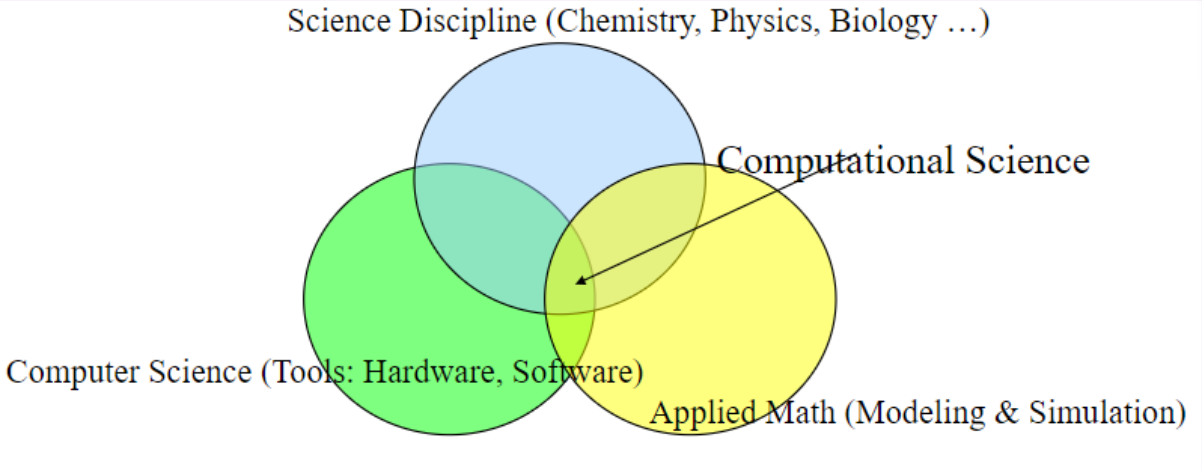
\includegraphics[width=0.8\textwidth]{images/computational_science_venn.png}
 \caption{Computational Science at the Intersection of Disciplines}
 \label{fig:computational_science_venn}
\end{figure}

Figure~\ref{fig:computational_science_venn} illustrates computational science as the intersection of three fundamental academic disciplines, forming a tripartite approach that defines the field's unique character and capabilities.

\subsubsection{The Three Foundational Disciplines}

\textbf{Science Disciplines} form the blue circle in our diagram, encompassing fields like chemistry, physics, biology, economics, and other domain sciences. These disciplines provide the fundamental questions that drive computational research and the real-world knowledge needed to validate computational results. For example, when studying climate change, atmospheric physicists provide understanding of weather patterns, while chemists contribute knowledge about greenhouse gas interactions in the atmosphere.

\textbf{Computer Science} represents the green circle, contributing the tools and methodologies for computation. This includes hardware design, software development, algorithms, and data structures that make complex calculations possible. Consider how computer scientists developed parallel processing algorithms that allow climate models to run efficiently on supercomputers, processing millions of calculations simultaneously.

\textbf{Applied Mathematics} forms the yellow circle, providing the mathematical framework that transforms real-world phenomena into solvable equations. This discipline offers modeling techniques, numerical analysis, and optimization methods that bridge abstract mathematics with practical problem-solving. For instance, mathematicians develop differential equations that describe how heat flows through the atmosphere, which can then be solved computationally.

\subsubsection{The Intersection: Where Innovation Happens}

The magic of computational science occurs at the center where all three circles overlap. This intersection creates a new discipline that is greater than the sum of its parts. A computational scientist studying drug discovery, for example, must understand the biological mechanisms of disease (science), implement machine learning algorithms to analyze molecular data (computer science), and develop statistical models to predict drug effectiveness (applied mathematics).

This interdisciplinary approach enables computational scientists to tackle problems that no single field could address alone. Weather prediction requires atmospheric science knowledge, sophisticated algorithms to process satellite data, and complex mathematical models—all working together to forecast tomorrow's conditions. The strength of computational science lies not in deep specialization within one field, but in the ability to synthesize knowledge across disciplines to solve complex, real-world problems.

\subsection{Real-World Applications Across Disciplines}

\begin{figure}[h]
 \centering
 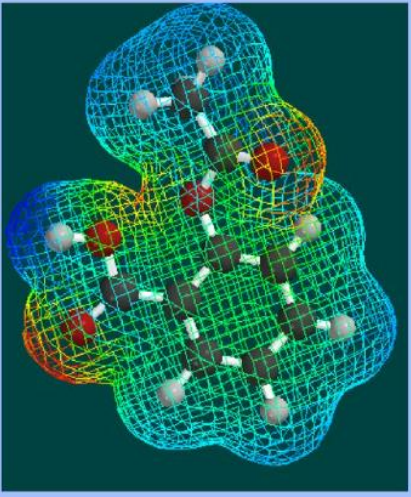
\includegraphics[width=0.6\textwidth]{images/molecular_structure.png}
 \caption{Computational Modeling of Molecular Structures}
 \label{fig:molecular_structure}
\end{figure}

The true power of computational science becomes evident when we examine its diverse applications across multiple scientific domains. Figure~\ref{fig:molecular_structure} illustrates one such application—the computational visualization of molecular structures that enables scientists to understand complex chemical interactions at the atomic level.

\subsubsection{Chemistry: Electronic Structure Determinations}

In computational chemistry, scientists use quantum mechanical calculations to determine how electrons are arranged around atoms and molecules. This electronic structure determination helps predict chemical reactions, design new materials, and understand molecular behavior. For example, pharmaceutical companies use computational methods to predict how drug molecules will interact with proteins in the human body, significantly reducing the time and cost of drug development compared to traditional laboratory experiments alone.

\subsubsection{Physics: Astrophysics and Galaxy Simulations}

Computational physics enables scientists to simulate cosmic phenomena that span billions of years and vast distances. Galaxy formation simulations help astronomers understand how the universe evolved from the Big Bang to its current state. These simulations combine gravitational physics, thermodynamics, and stellar evolution models to recreate the birth and death of stars, the formation of galaxies, and the large-scale structure of the universe—phenomena impossible to observe directly due to their immense time scales.

\subsubsection{Biology: Population Dynamics}

Computational biology models help scientists understand how populations of organisms change over time. These models can predict the spread of infectious diseases, track endangered species recovery, or analyze ecosystem stability. During the COVID-19 pandemic, computational epidemiological models became crucial tools for predicting infection rates and evaluating the effectiveness of public health interventions.

\subsubsection{Environmental Science: Acid Rain Deposition Models}

Environmental scientists use computational models to track how pollutants move through the atmosphere and affect ecosystems. Acid rain models simulate how sulfur and nitrogen compounds travel from industrial sources, undergo chemical transformations in the atmosphere, and eventually deposit in forests and lakes. These models help policymakers understand the regional impacts of pollution and design effective environmental regulations.

\subsubsection{Political Science and History: Analyzing Complex Social Phenomena}

Computational social science applies quantitative methods to understand historical events and political processes. For instance, researchers have used computational models to analyze the causative factors in the Bosnian War conflict, examining how ethnic tensions, economic factors, and political decisions interacted to escalate the situation. These models help historians and political scientists identify patterns and test theories about complex social phenomena.

\subsubsection{Medicine: Epidemiology and Pharmacokinetics}

Medical applications of computational science range from tracking disease outbreaks to modeling how drugs move through the human body. Epidemiological models help public health officials predict and control disease spread, while pharmacokinetic models help doctors determine optimal drug dosages by predicting how medications are absorbed, distributed, metabolized, and eliminated by the body. These computational tools have become indispensable for evidence-based medical practice.

The diversity of these applications demonstrates that computational science is not confined to traditional "hard" sciences but extends to any field where complex systems can be modeled mathematically and solved computationally. Each application requires the same tripartite integration of domain expertise, computational methods, and mathematical modeling that defines computational science as a discipline.


